\chapter{Implementation}
\label{ch:implementation}

% Budget and sources: docs/thesis/outline.md. Every claim about behaviour points at a test, a figure or a number in data/.

% Sections are written as the work lands; order follows the outline, so earlier sections are filled in later.
\section{The service and its persistence}
\label{sec:impl-service}

The engine is one Go program. It uses the standard library's HTTP server and router and nothing above them, so
every behaviour that wraps a request is a small piece of code in the repository rather than a framework's
convention: recovery from a panic, a request identifier, a structured log line, and, for the operations that need
them, authentication, the rate limit and validation against the contract. The server sets explicit timeouts for
reading, writing and idle connections, and on a termination signal it stops accepting requests, lets the ones in
flight finish and flushes its telemetry before it exits. The code follows the layers of the design. The
\code{dispute} context has a pure domain layer with no input or output at all, which is why chapter~\ref{ch:design}
can describe the state machine, the clocks and the ledger as functions; an application layer of use cases that
orchestrate it; infrastructure adapters for the database, the mail relay and the simulated core; and HTTP ports
that implement the generated interface. A shared platform package holds what has no domain knowledge, such as
configuration, errors, telemetry and the database pool.

PostgreSQL is the only stateful dependency, and that was a decision rather than a default. Every mechanism that
is often given its own system lives in the database instead, inside the same transaction and the same trace as the work
it serves: the idempotency store, the per-tenant rate-limit counters, the analysts' sessions, the outbox of
emails, and the one-at-a-time lock for background sweeps. A second system would be added when a measurement, not a
preference, shows the database to be the bottleneck for one of them, and the evaluation found its queries well
under a millisecond at the 95th percentile (section~\ref{sec:eval-latency}). A dispute is stored as a row holding
its current state and a version, beside an append-only log of every transition with its actor, payload, the
idempotency key that caused it and the trace of the request. A transition reads the row, runs the state machine in
memory and writes back only if the version is still the one it read; a concurrent writer that got there first
makes the write affect no row, and the caller receives a conflict instead of waiting on a lock. A unique index on
the dispute and its sequence number guards the same rule a second time.

The 83 queries are written in SQL and compiled into typed Go functions, so a column renamed in a migration breaks
the build rather than a request. The 24 migrations run forward only, embedded in the binary and applied by a
separate command under the schema owner's role; the service checks the schema version when it starts and refuses
to serve behind it. The service itself connects as a login that can read and insert where it must and cannot
alter the schema or rewrite the event log, which is what the tests of section~\ref{sec:eval-log} rely on.
Identifiers are time-ordered UUIDs generated in Go, so new rows land at the end of their indexes. The image that
ships contains the statically linked binary on a minimal base with no shell, running as an unprivileged user.

\section{One contract, two generated sides}
\label{sec:impl-contract}

Section~\ref{sec:design-failures} made one document the contract; this section is what that costs and buys in the
build. One command regenerates everything derived from it on the server: the typed queries from the SQL, and the
server interface, the request and response types and the validator from the OpenAPI document. A second command
regenerates and compares the result with what is committed, and fails with the list of files that differ, so the
check runs in continuous integration and on a developer's machine in the same way. On the client, a script reads
the same document and writes two files: the TypeScript types and request functions, and a validation schema for
every component schema in the document.

The two client files are generated independently, from different libraries, and could disagree. Each generated
schema is therefore followed by an assertion that the type it validates is exactly the type generated for the
same component (figure~\ref{fig:schema-pair}); a schema that drifted from its type is a compile error, not a
surprise in a form. The workbench validates in one place only: a module that accepts any schema in the common
Standard Schema interface, adapts the generated ones behind it, and returns either the value or one error per
field. Forms use it before they submit, and every server function uses it on its input before it calls the
engine, so a malformed request is refused at the edge of each side even though both sides would refuse it anyway.

\begin{figure}[htbp]
\begin{lstlisting}
# docs/api/openapi.yaml
CreateDisputeRequest:
  type: object
  required: [transactionId]
  properties:
    transactionId: { type: string, format: uuid }
    reason: { $ref: "#/components/schemas/DisputeReason" }
    suggestion: { $ref: "#/components/schemas/AcceptedSuggestion" }

// frontend/src/api/schemas.gen.ts (generated)
export const CreateDisputeRequest = Type.Object({
  transactionId: Type.String({ format: 'uuid' }),
  reason: Type.Optional(DisputeReason),
  suggestion: Type.Optional(AcceptedSuggestion),
})
export type CreateDisputeRequest = Static<typeof CreateDisputeRequest>
const _CreateDisputeRequest: Same<CreateDisputeRequest,
  components['schemas']['CreateDisputeRequest']> = true
\end{lstlisting}
\caption{One component of the contract (descriptions omitted) and the validation schema generated from it. The
last line compiles only if the schema's type equals the type generated for the same component.}
\label{fig:schema-pair}
\end{figure}

\section{Sessions and sign-in}
\label{sec:impl-sessions}

An analyst reaches the workbench through their institution's front door, an address ending in the tenant's short
name. An unauthenticated visit there starts the authorization-code flow with proof-key protection against that
tenant's realm and remembers the page that was asked for, restricted to the workbench's own paths. The callback
validates the identity token, creates a new session identifier and gives the browser a cookie carrying only that
identifier, which scripts cannot read and which the browser does not attach to requests other sites make in the
background. The tokens
themselves stay on the server.

The session needed somewhere to live, and the workbench has no database connection of its own. It seals the
session's contents, the analyst's identity and tokens, with authenticated encryption under a key only the
workbench server holds, and stores the sealed result through internal endpoints of the engine that accept a
service key rather than a tenant's credential. The engine keeps the ciphertext and an expiry, enforces the expiry
on every read and sweeps expired rows, but cannot read what it stores; neither can anyone holding a copy of the
database. Every page renders on the server with the session's access token, and every later action is a server
function that reads the same token on the server, so the browser never sees a token at all.

Tokens are refreshed only on the server. When a refresh fails, the browser is sent back through the front door,
which signs the analyst in again silently while their session with the identity provider lasts, so a long-open tab
recovers instead of showing an error. A session ends in one of four ways: the analyst signs out, which also ends
the identity provider's session; thirty minutes pass without activity; ten hours pass in total; or the identity
provider tells the workbench directly, by back-channel logout, that the analyst was signed out elsewhere or
disabled, which ends every workbench session belonging to them.

\section{The analyst workbench}
\label{sec:impl-workbench}

The workbench is the only part of the system a person touches, and the decision that shapes it is
that the browser is never given a credential. Every call the interface makes is a
\emph{server function}: the code is written beside the component that needs it, but it executes on
the workbench's own server, which reads the sealed session cookie, exchanges it for the analyst's
access token and calls the service. A token therefore never reaches a script, and no bearer value
is available to be read out of storage; the browser suite asserts exactly that, failing if
anything resembling a token appears in \code{localStorage} or \code{sessionStorage}. The cost is
one network hop that a direct client would not pay, and the benefit is that the credential surface
of the service stays the two kinds described in section~\ref{sec:design-tenancy}: a key for a
tenant's own systems, and a realm token for a person.

Data is fetched through one query definition per domain, keyed by the arguments it was given, so
that the key is the single place a cache entry is named. Each definition ends with the same
transformation, which maps the contract's problem document onto the client failure taxonomy of
section~\ref{sec:design-failures}; a page therefore renders a refusal rather than discovering an
exception. Writing follows the same route in reverse. Forms are built from the TypeBox schemas
that the contract already generates, so the structural rules the service enforces are the rules
the form applies before it submits, and a validation refusal that names a field is placed back on
that field, indistinguishable to the analyst from one the browser found itself. Every other kind
of failure stays in the mutation and is rendered once, as a banner. Validation itself is reached
through one library-neutral interface, Standard Schema, with TypeBox adapted behind it, so the
schema library can be exchanged without touching the code that validates.

What the analyst sees is a grid and a small number of panels (figure~\ref{fig:workbench}). The
dispute list carries the actions and the filter on a toolbar above it and its paging controls
below, and the page that a dispute opens onto is a stack of panels, one per concern: the summary,
the fraud score and its signals, the regulatory clocks with their legal basis, the actions the
state machine currently allows, the ledger, the letters and emails sent, and the event log
(figure~\ref{fig:dispute}). The actions offered are not a fixed menu; they are the transitions the
service reports as allowed for that dispute in that state, so the interface cannot offer a move
the domain would refuse.

Paging is worth one honest note. The list is keyed on a cursor rather than an offset, which keeps
the query cheap and stable while rows are being inserted, but a cursor carries no notion of how
many rows exist. The pager therefore counts the pages it has walked and can always return to the
first, and it deliberately offers no jump to the last page and no total, because the only way to
show either would be a counting query over the whole tenant's disputes on every page turn.

An organisation and a person are both allowed a picture. The tenant's logo and the analyst's own
are stored in tenant-scoped tables under the same row-level security policy as every other
tenant-owned row, capped at 256 kB, and accepted only as PNG, JPEG or WebP. SVG is refused on
purpose: it is a document that can carry script, and it would be served from the service's own
origin. A tenant administrator may replace the organisation's logo, whereas a picture belongs to
whoever is signed in and needs no role at all; a tenant key is refused, since there is no person
behind it.

\begin{figure}[htbp]
\centering
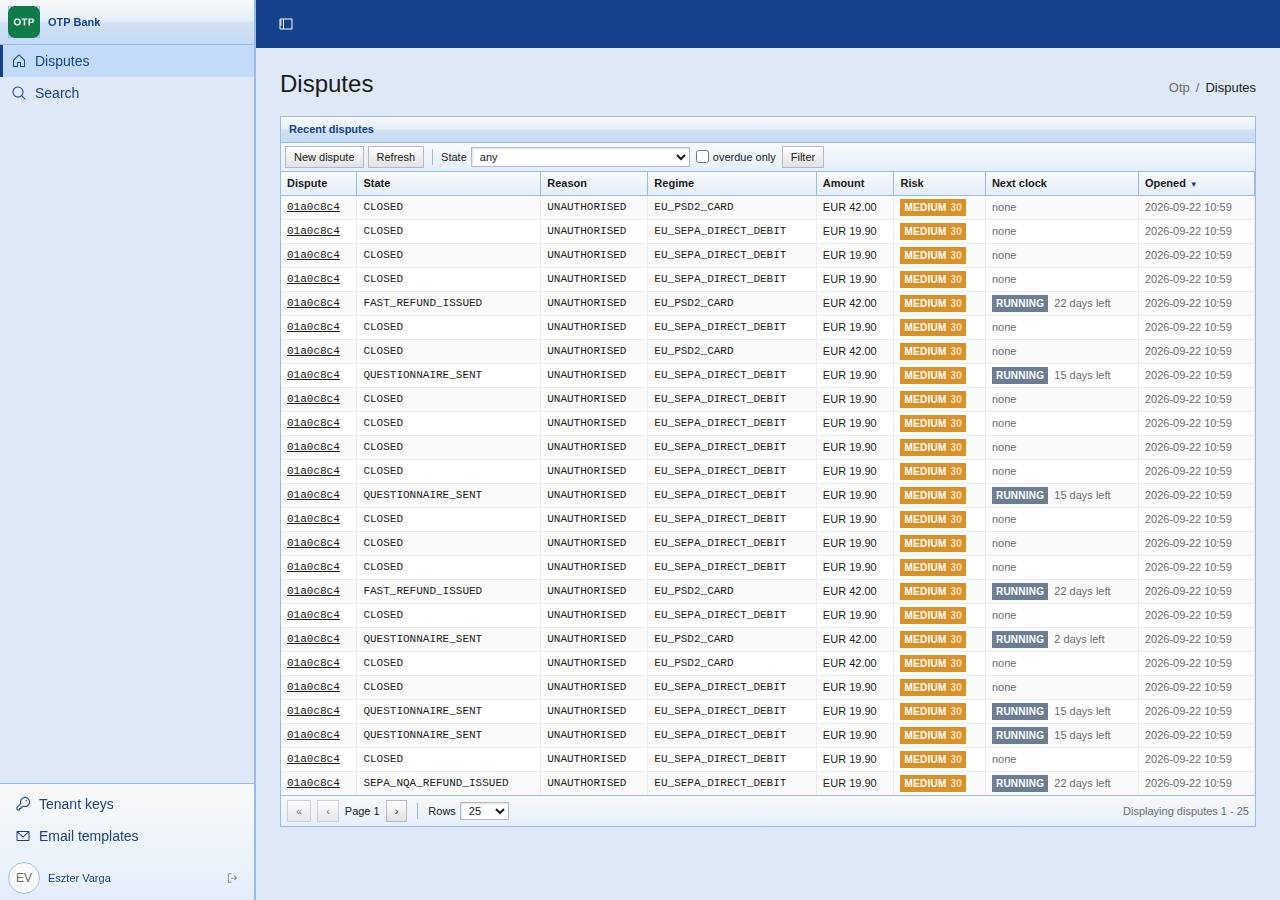
\includegraphics[width=\textwidth]{workbench.jpg}
\caption{The workbench: the organisation and the signed-in analyst on the left, the dispute grid
with its toolbar and pager on the right. Captured against the local stack by
\code{pnpm screenshot}, so it can be retaken after a change rather than going stale.}
\label{fig:workbench}
\end{figure}

\begin{figure}[htbp]
\centering
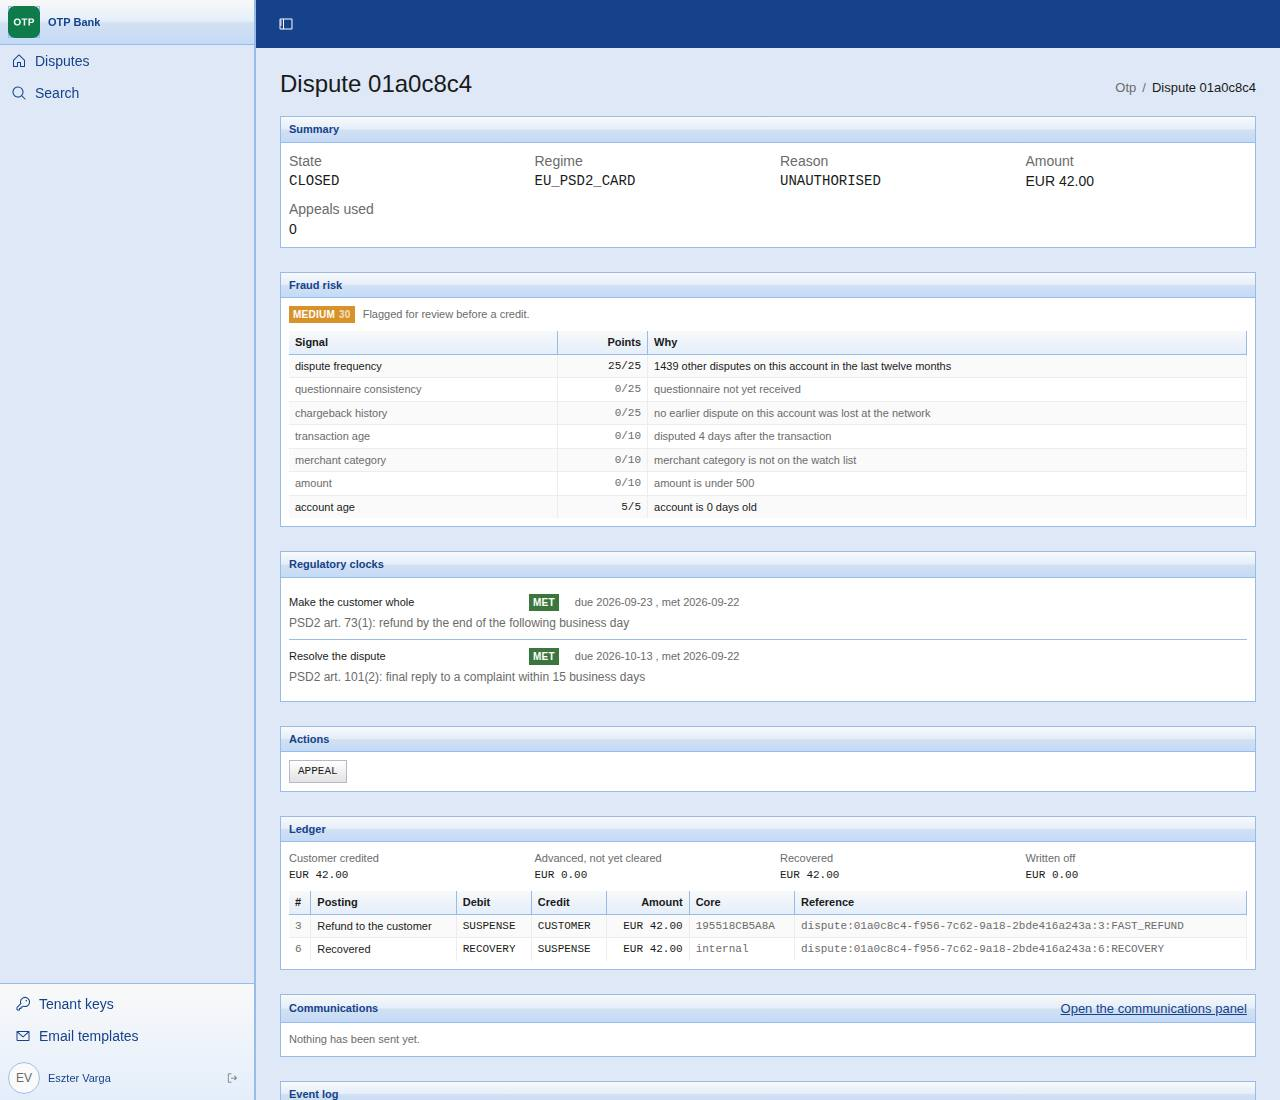
\includegraphics[width=\textwidth]{dispute.jpg}
\caption{One dispute: the summary, the fraud score with the signals that produced it, the
regulatory clocks with their legal basis, and the transitions the state machine allows from the
current state.}
\label{fig:dispute}
\end{figure}

\section{Proposals from a typed-decision model}
\label{sec:impl-decisions}

Three places in the workbench turn a person's prose into a value the domain already has a type for.
An intake describes a problem and someone picks one of four reasons. A customer answers a
questionnaire in a paragraph and an analyst records typed answers. An analyst wants a list and
types a sentence rather than setting three filters. A \emph{typed decision model} answers exactly
that shape: it takes a state and questions whose answers are constrained to a closed set, and
returns the value with a probability in one pass, generating no text, so there is nothing to parse
and no free-form output to police.

The model sits behind a port in the application layer beside the banking core of
section~\ref{sec:design-core}, and for the same reasons: it is someone else's system, it can be
slow, it can be down, and the domain must not know which one it is. The rule that governs its use
is that it proposes and a person disposes. No transition, no clock, no posting and no letter may
depend on it; every use is a field that arrives filled in and can be changed before anything is
recorded; and what is stored is always the value the person left. The port is optional, so with no
model configured each of these fields is simply empty and the engine behaves as it did before,
which is also what keeps the claim of section~\ref{sec:impl-service} about a single stateful
dependency honest. A proposal below three quarters probability is dropped rather than shown,
because a wrong pre-filled answer costs an analyst more attention than an empty one.

Two failures found by driving the real model, rather than by testing against a fake, shaped the
design more than the benchmark did. A question offering only the four reasons must answer with one
of them: a message reading ``hello I have a question about my account'' came back as an
unauthorised payment at 0.81, comfortably above the gate. The question now offers an explicit
option for text that describes no dispute at all, and that message yields nothing. The same problem
has a different shape for yes and no questions, which cannot abstain: asked about a message that
answers nothing, the model returned a confident negative to every question on the questionnaire.
The batch now carries a gate question asking whether the message is a customer answering about a
disputed payment, and without it nothing is proposed. A forced choice, in other words, is a
proposal generator whether or not there is anything to propose, and the remedy is to give the model
somewhere to put its uncertainty rather than to raise the threshold.

Whether any of this helps is one number, and the system records it. When an analyst opens a dispute
from a proposed reason, the opened event carries what was proposed, how sure the model was, and
whether they kept it, beside the reason they actually chose. The audit trail therefore stays a
record of what a person did, with the machine's contribution visible next to it, and the acceptance
rate becomes something the running system reports rather than something the author asserts.

\section{Observability from day one}
\label{sec:impl-observability}

Telemetry was part of the first commit, because a system whose behaviour is regulated must be able to show what it
did, and because instrumentation added late tends to cover what was easy rather than what matters. Both services,
the engine and the workbench server, use OpenTelemetry and are configured only through the standard environment
variables; without them they still create every span and metric but export nothing, so a developer's run stays
quiet. Every request is a span named after its route pattern rather than its address, which keeps the number of
distinct names bounded by the routing table. Every database statement is a child span named after its query, with
no values recorded. Logs go to standard output and, with the trace's identifiers attached, to the same backend as
the traces, after a redaction step that runs before any destination.

A request from the workbench is one trace across both services: the workbench server opens a span per request and
per server function, and its calls to the engine carry the trace context, so the engine's spans join it without
any change on that side. There is deliberately no instrumentation in the browser, since the trace already starts
at the first thing the page talks to. Work that happens later is its own trace, linked to the request that caused
it rather than nested inside it: each queued email stores the trace context of the transition that owed it, and
its delivery, minutes or hours later, links back. Nothing in an attribute carries a credential or a customer's
personal data.

Locally the signals land in a Grafana stack started with the rest of the system, which provisions two dashboards,
one per service, and three alert rules from the repository: more than one percent of responses failing with a
server error, a 99th-percentile latency above one second, and an outbox that is not draining. The rules alert on
symptoms a user would notice rather than on causes such as processor or memory use, which are diagnostics. A
synthetic probe keeps a trickle of realistic traffic flowing so that no panel is ever empty, and the evaluation of
chapter~\ref{ch:evaluation} reads its latency numbers back from these same metrics rather than from a separate
harness. An operator's guide in the repository explains each panel, which signal answers which question, and four
worked situations taken from a real run.

\section{Review and release discipline}
\label{sec:impl-ci}

Every change reached the main branch as a pull request, squashed into one commit whose message is the pull
request's title and body; by the time of writing that was 95 merged pull requests and 28 decision records. The
branch is protected by a ruleset that forbids direct pushes, force pushes and deletion, requires a linear history
and signed commits, and requires eight checks to pass on a branch that is up to date with the main branch, so a
change is always tested against what it will actually be merged into. A pull request's body follows a fixed
template of type, a two- or three-sentence description of its effect, whether it includes tests, how it rolls out
and which decision record it implements, and one of the eight checks rejects a body that does not.

Continuous integration runs one job per area, with a named step per check, so a failure names its cause. The
backend job checks formatting, that generated code is current, static analysis, the linter, that the module files
are tidy, the dependency vulnerability database, and that the authorization policies validate against their
schema. The backend test job runs the unit and database-backed suites with the race detector against a real
PostgreSQL service, and comments the coverage on the pull request beside that of the main branch. The image job
builds the backend image and smoke-tests it the way a deployment would run it: migrations as the owner, then the
service as its least-privileged login, until the readiness endpoint answers. The frontend job generates, type-checks,
lints, looks for dead code, checks formatting, runs the tests, reports coverage and builds, and the frontend image
is built and smoke-tested in the same way as the backend's. The browser suite runs as its own workflow on every
pull request that touches the application and on the main branch, and reports, but never gates a merge, because a browser test that is flaky for
reasons outside the change would otherwise teach everyone to ignore red.

The same checks run locally with one command before every push, and a pre-commit hook formats and lints the files
being committed. Dependencies are watched weekly across the Go module, the frontend packages, the workflows and the
container images, and arrive as pull requests through the same gate. The two vulnerability advisories published
against the Go toolchain during the writing of this chapter show the gate working as intended: the vulnerability
check failed on every open pull request until a separate one moved the toolchain to the fixed release. Releasing
ends at the images: they are built, smoke-tested and reproducible from any commit on the main branch, and the
deployment they would go into is outside the scope of this thesis (section~\ref{sec:req-scope}).
